
%____________________DOCUMENT PREAMBLE_________________________________
\documentclass[12pt]{report}
\usepackage{appendix}
\usepackage{graphicx}
\usepackage{sidecap}
\usepackage{wrapfig}
\usepackage{float}
\usepackage{supertabular}
\usepackage{array}
\usepackage{threeparttable}
\usepackage{booktabs}
\usepackage[margin=3cm]{geometry}
\usepackage{setspace}
\usepackage{url}
\usepackage{amssymb}
\usepackage{amsmath}
\usepackage[version=3]{mhchem}  %Chemical compounds \ce{(NH4)2SO4}.
%\usepackage{fixltx2e}
\usepackage{indentfirst}
\usepackage{subcaption}
\usepackage{caption}
\usepackage{pdflscape}
\usepackage{lipsum}
\usepackage{blindtext}
%\usepackage[nottoc]{tocbibind} %So bibliography won't appear as a chapter in the document
\usepackage{pgfplots}
\usepackage{fancyhdr}
\usepackage{pgfplotstable}
\usepackage{colortbl}
\usepackage{xcolor}
\usepackage{multirow}
\usepackage{tocloft}
\usepackage{notoccite} % PREVENTS CITES IN CAPTIONS FROM MISNUMBERING YOUR REFERENCES https://tex.stackexchange.com/questions/302594/citation-inside-a-caption-dont-follow-order-of-appearance
\pgfplotsset{compat=1.7}
\usepackage{tikz}
\renewcommand{\bibname}{References} % or other title eg. Bibliography
\bibliographystyle{ieeetr} %styles: abbrv, acm, alpha, apalike, ieeetr, plain, siam, unsrt.
\usepackage[numbers,sort&compress]{natbib}
\renewcommand{\cftchapleader}{\cftdotfill{\cftdotsep}} %dots for chapters
\hbadness=99999

%_______________________________________________
%TO CREATE LIST OF APPENDICES

\newcommand{\listexamplename}{List of Appendices}
\newlistof{example}{exp}{\listexamplename}
\newcommand{\example}[1]{%
\refstepcounter{example}
\par\noindent\textbf{Appendix \theexample. #1}
\addcontentsline{exp}{example}
{\protect\numberline{\thechapter.\theexample}#1}\par}

\makeatletter
\@addtoreset{example}{chapter}
\makeatother
%from https://texblog.org/2008/07/13/define-your-own-list-of/
%_____________________________________________________________

\begin{document}
\frenchspacing %override to remove double space after periods.

%__________   TITLE PAGE   _________________________________________



%__________   TITLE PAGE   ________________________________


\thispagestyle{empty}
\begin{center}
\begin{singlespace}
\textbf{Increasing Sensitivity to Emerging Jets in CMS Through Novel Triggering Algorithms}
\end{singlespace}
\vspace{4 mm}
by
\\
\vspace{4 mm}
Roy F. Cruz Candelaria % WRITE YOUR NAME HERE
\vspace{4 mm}
\begin{singlespace}
A thesis submitted in partial fulfillment of the requirements for the degree of %CHANGE: proposal, thesis, or dissertation
\end{singlespace}
\vspace{4 mm}
MASTER OF SCIENCE % WRITE YOUR DEGREE HERE
\\
in
\\
Physics % WRITE YOUR DISCIPLINE HERE
\\
\vspace{4 mm}
\begin{singlespace}

UNIVERSITY OF PUERTO RICO
\\
MAYAG\"UEZ CAMPUS
\end{singlespace}

2025 % WRITE YEAR
\end{center}
\bigskip
\bigskip
\bigskip
\bigskip
\bigskip
\bigskip
\bigskip

%_______________________FIRMAS__________________________________________________
  \noindent Approved by:
\\
\\

  \noindent
\line(1,0){200} \hspace{40 mm} \line(1,0){100}\\
  \noindent
\vspace{-1.75\baselineskip}
  \begin{tabbing}
Longest Professor Name Here Longest Professor Name Here, Ph...D. \=  \kill 
Sudhir Malik, Ph.D. \>  Date\\President, Graduate Committee  %CHANGE PROFESSOR NAME HERE
\end{tabbing}



  \noindent
\line(1,0){200} \hspace{40 mm} \line(1,0){100}\\
  \noindent
\vspace{-1.75\baselineskip}
  \begin{tabbing}
Longest Professor Name Here Longest Professor Name Here, Ph...D. \=  \kill 
Edgardo Marrero, Ph.D. \>  Date\\Member, Graduate Committee  %CHANGE PROFESSOR NAME HERE
\end{tabbing}


  \noindent
\line(1,0){200} \hspace{40 mm} \line(1,0){100}\\
  \noindent
\vspace{-1.75\baselineskip}
  \begin{tabbing}
Longest Professor Name Here Longest Professor Name Here, Ph...D.   \=  \kill 
Samuel Santana, Ph.D. \>  Date\\Member, Graduate Committee %CHANGE PROFESSOR NAME HERE
\end{tabbing}



  \noindent
  \line(1,0){200} \hspace{40 mm} \line(1,0){100}\\
  \noindent
\vspace{-1.75\baselineskip}
  \begin{tabbing}
Longest Professor Name Here Longest Professor Name Here, Ph...D.  \=  \kill 
FirstName I. LastName, Ph.D. \>  Date\\Department Chairperson  %CHANGE PROFESSOR NAME HERE
\end{tabbing}  %decide if you have a 3, 4 or 5-member committee.
\newpage

%____PRELIMINARY PAGES: COPYRIGHT, ABSTRACT, ACKNOWLEDGMENTS, DEDICATION________

\pagenumbering{roman}
\setcounter{page}{2}
\doublespacing




%__________   ABSTRACT ENGLISH ________________________________
\vspace*{0.5in}
\begin{center}
	\section*{ABSTRACT}
\end{center}
%\addcontentsline{toc}{section}{ABSTRACT} %para que aparezca en la tabla de contenido

\noindent
Hi! We encourage you to visit https://libguides.uprm.edu/writingclinics and check out the \textbf{Abstracts Clinic.} Keep in mind that depending on your discipline, abstracts should be a \textbf{single paragraph}, containing no more than \textbf{150 words} for theses or \textbf{350 words} for dissertations. It should concisely but clearly summarize your thesis document. The \textbf{IMRaD format} is recommended for writing abstracts: Introduction (1-3 sentences long, present tense), Methodology (1-3 sentences long, past tense), Results (1-3 sentences long, past tense), and Discussion (1-2 sentences long, present tense). Remember that the number of sentences and verb tense are only guidelines!


%____________________________________________________________





\newpage




%__________   ABSTRACT ESPANOL  ______________________________

\vspace*{0.5in}
\begin{center}
	\section*{RESUMEN}
\end{center}
%\addcontentsline{toc}{section}{RESUMEN} %para que aparezca en la tabla de contenido

\noindent
El Resumen debe ser una traduccion del Abstract. No deben diferir en contenido. % PASTE YOUR RESUMEN HERE (DELETE \blindtext)
%____________________________________________________________
 %edit abstract.tex

%_______________COPYRIGHT PAGE___________

\vspace*{7in}
\begin{center}
Copyright \copyright
\\
Your Name Here %%%
\\
20XX
\end{center}
\pagebreak
%_____________________________________________




%__________   DEDICATION  ______________________________
\vspace*{2in}
\begin{center}
	\emph{Para mi mamá y mi hermano.}
\end{center}
%____________________________________________________________

\newpage


%__________   ACKNOWLEDGMENTS  ______________________________
\vspace*{0.5in}
\begin{center}
	\section*{ACKNOWLEDGMENTS}
\end{center}
%\addcontentsline{toc}{section}{ACKNOWLEDGMENTS}


% \noindent I want to thank the GRIC personnel! :D
% \newline
% \noindent
% \blindtext % PASTE YOUR ACKNOWLEDGMENTS HERE (DELETE \blindtext)

\noindent The journey that led to the completion of this work would not have been possible without the love and support of my mother, Ofelia Candelaria, and my brother, Ed Ralph. I will never be able to repay their unwavering support and encouragement throughout. Their belief in me has been a constant source of motivation and strength. Moreover, their dedication and sacrificial efforts in their own fields offered examples of excellence which I will continue to strive to emulate.

I extend my deepest gratitudes towards Sudhir Malik. His guidance and mentorship have been invaluable to me, and I hope to pay forward the support he has shown me to the next generation of high energy physicists. Furthermore, I am deeply grateful to Kevin Pedro, Gabriele Benelli and the LHC Physics Center (LPC) at Fermilab for their guidance. The expertice they shared was instrumental in the completion of this work and in my growth as a physicist.

This work would not have been possible without the support of funding from the National Science Foundation (NSF) through the grant PHY-2111134 ("Physics Beyond Standard Model with the CMS Pixel Detector") and the LPC's Guest \& Visitor Program which allowed me to conduct much of the work presented here at Fermilab.

Finally, I wish to dedicate this work to the loving memory of Moti \& Shiba. I will forever cherish the pure love \& joy they brough into my life.

%____________________________________________________________
 %dedication and acknowledgment, edit acknowledgment.tex
\newpage

%_____________set TOC and subsection depth___________________________________

\setcounter{tocdepth}{3}
\setcounter{secnumdepth}{3}
%____________________________________________________________________________

\tableofcontents			
 \cleardoublepage
  \addcontentsline{toc}{section}{\listfigurename}\listoffigures

  \cleardoublepage
  \addcontentsline{toc}{section}{\listtablename}\listoftables



\chapter*{List of Acronyms}

\noindent
\vspace{-1.75\baselineskip}
\begin{tabbing}
	LONGEST \=  \kill %change LONGEST to be the longest acronym you have

	CMS 	\> Compact Muon Solenoid\\
	LHC 	\> Large Hadron Collider\\
	EMJ 	\> Emerging Jet\\
	SVJ 	\> Semi-Visible Jet\\
	LLP 	\> Long-Lived Particle\\
	DM 		\> Dark Matter\\
	BSM 	\> Beyond the Standard Model\\
	SM 		\> Standard Model\\
	DS 		\> Dark Sector\\

\end{tabbing}
 %edit acronyms.tex
\addcontentsline{toc}{section}{List of Acronyms}


\chapter*{List of Symbols}

\noindent
\vspace{-1.75\baselineskip}
\begin{tabbing}
	LONGEST \=  \kill %change LONGEST to be the longest symbol you have


	kg \>  kilogram\\ %ADD MORE SYMBOLS HERE
	$\tau$ \>tau\\
	$\mu$L \> microliters\\




\end{tabbing}

\addcontentsline{toc}{section}{List of Symbols}
\addcontentsline{toc}{section}{\listexamplename}\listofexample


\newpage
%%%% PAGE NUMBERING ___________

%%%% page number location at bottom right______________________________________________________
% move page number to right on first page of Chapter
\fancypagestyle{plain}{%
\fancyhf{} % clear all header and footer fields
\fancyfoot[R]{\thepage} % except the right
\renewcommand{\headrulewidth}{0pt}
\renewcommand{\footrulewidth}{0pt}}

% move page number to right on rest of pages
\pagestyle{fancy}
\fancyhf{}                         %to change headers and footers
\renewcommand{\headrulewidth}{0pt} % to default to no line in header
\rfoot{\thepage}                   %to move page number to bottom right

\pagenumbering{arabic}
%%_________________________________________________________________________________




\chapter{Introduction}  
\section{Motivation, Purpose, Justification}

\noindent Hi! We encourage you to visit https://libguides.uprm.edu/writingclinics. The GWF Writing Clinics provide in-depth, useful information for preparing: abstracts, literature reviews, citations (Mendeley), academic writing, thesis outline, grammatically-sound writing, presentations (communication strategies in oral presentations and poster sessions) and visual design.  %Dummy text. Replace with your text.

\section{Objectives, Research Questions, Hypothesis}


\noindent Example of bullet items. Mention objectives, research questions, or hypotheses:
\begin{itemize}
\item Analyze
\item Study 
\item Identify
\item Construct
\item Analyze 
\end{itemize}
	
\noindent Example of numbered items. The work is divided in three phases: 

\begin{enumerate}
\item Collect data
\item Build model
\item Validate results
\end{enumerate} 


\section{Chapter Summary}

\noindent
This is how you add indented descriptive paragraphs. This thesis consists of 6 chapters which are briefly summarized below:
\begin{description}
\item [Chapter 1:] Discusses project justification and objectives. Serves as an introduction to the investigation. \lipsum[1][5-7]
\item [Chapter 2:] Presents an overview of \lipsum[1][5-7]
\item [Chapter 3:] Provides a means of presenting the \lipsum[1][5-7]
\item [Chapter 4:] Discusses what a \lipsum[1][5-7]
\item [Chapter 5:] Presents a simulation model for \lipsum[1][5-7]
\item [Chapter 6:] Presents Results for \lipsum[1][5-7]
\item [Chapter 7:] Makes final remarks regarding the study and proposes several ideas for future work.
\end{description}




\chapter{The CMS Experiment at the Large Hadron Collider}  

\section{How to add sections/subsections to your \LaTeX\ document}


\noindent \LaTeX\ provides three levels of nested subsections by using the commands \textbf{section, subsection and subsubsection.} %WRITE HERE

\section{Section A}
\noindent \lipsum[1][1] %WRITE HERE

\subsection{Subsection A}
\noindent \lipsum[1][1] %WRITE HERE

\subsubsection{Subsubsection A}
\noindent \lipsum[1][1] %WRITE HERE




\chapter{Monte Carlo Generation}  

\noindent You can visit the Overleaf Documentation library at: https://www.overleaf.com/learn or the official \LaTeX\ wiki at: \textbf{https://en.wikibooks.org/wiki/LaTeX} for in-depth guides to the \LaTeX\ typesetting system.

\section{How to incorporate citations in your document}


\noindent Make sure you have your references file in \textbf{.bib format}. You can export it from Mendeley and copy/paste them into the \textbf{referencias bib} file. Using the \textbf{citecommand}, start writing your source identifier and Overleaf will automatically show you the available references. A sample citation \cite{dirac}. If you want to cite two references \cite{einstein,knuth-fa} or \cite{einstein},\cite{knuth-fa}. Citing a range of references \cite{einstein,knuth-fa,radiation2}.


\subsection{Citation Styles}
\noindent There are several bibliography styles to choose from: \textbf{abbrv, acm, alpha, apalike, ieeetr, plain, siam, unsrt.} The default is ieeetr. Remember to change the option in the document preamble in \textbf{tesis.tex} %WRITE HERE


\section{Using Images}




%FIGURE  EXAMPLES___________________________________________________________________________

\noindent This is an example of a figure, as shown in Figure \ref{gric}. Your images must be uploaded to the \textbf{images} folder. Accepted file formats are \textbf{pdf, png, jpg, and eps}. Use the following options for the location of the image on the page: \textbf{[htbp]} that refer to here, top, bottom, or special page. Pay attention to the image width. If the image is wider than the margins, \LaTeX\ will produce an warning or error.

\begin{figure}[h]
\begin{center}
\includegraphics[width=0.3\textwidth]{images/GRIC} %specify width
\end{center}
\caption{GRIC logo!!} %specify caption
\label{gric}
\end{figure}

%


\subsection{Adding Subfigures}
\noindent If you need to place two subfigures in your figure, follow the example below:

\begin{figure}[h!]
\begin{subfigure}{.48\textwidth}
  \centering
  % include first image
  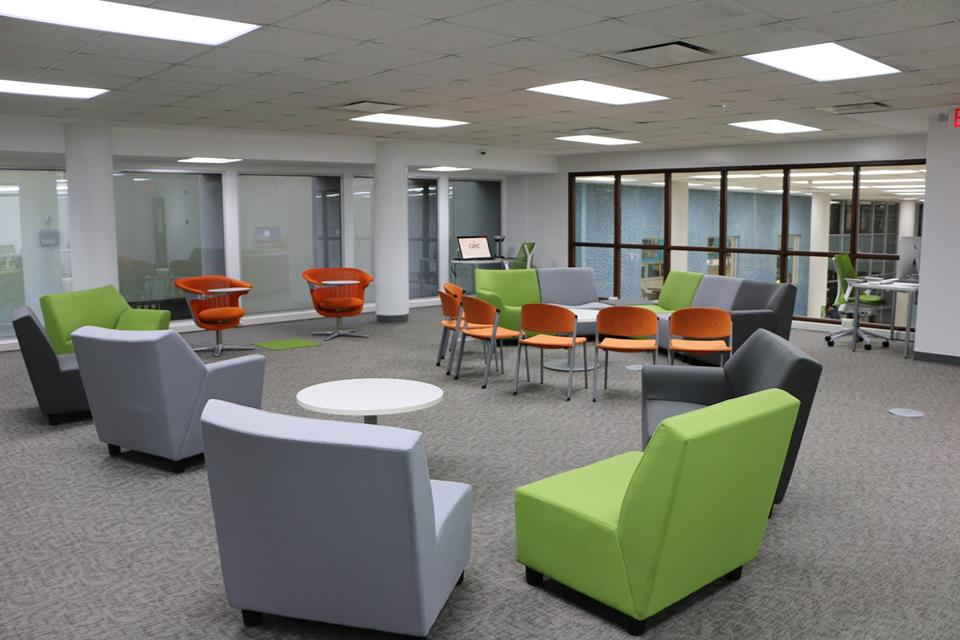
\includegraphics[width=.8\linewidth]{images/2}  
  \caption{Put your sub-caption here}
  \label{fig:sub-first}
\end{subfigure}
\begin{subfigure}{.48\textwidth}
  \centering
  % include second image
  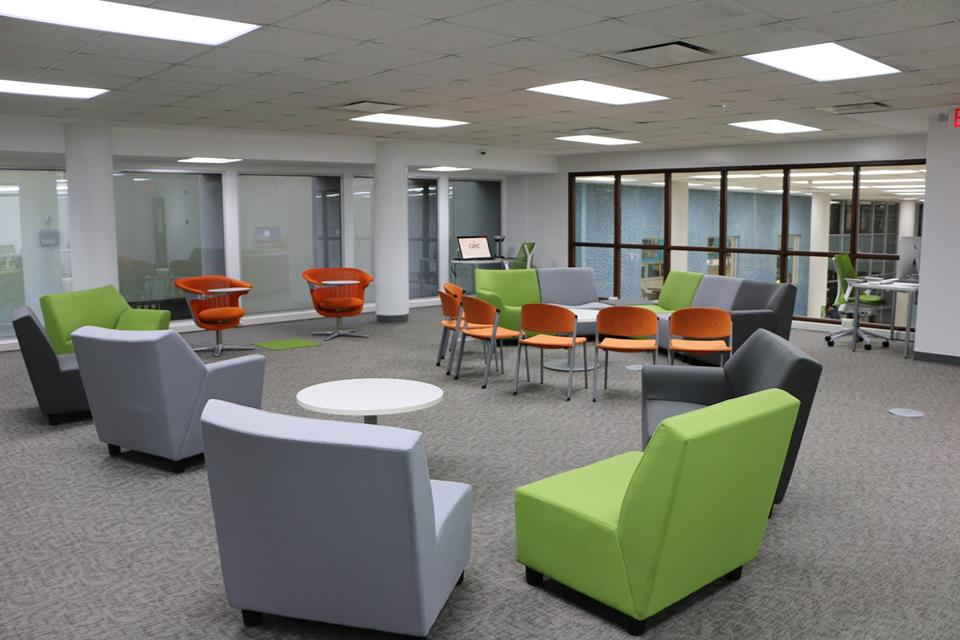
\includegraphics[width=.8\linewidth]{images/2}  
  \caption{Put your sub-caption here}
  \label{fig:sub-second}
\end{subfigure}
\caption{Put your caption here}
\end{figure}


\noindent If you need to place four subfigures in your figure, follow the example below, but \LaTeX\ is very particular with widths, so you have to play around with the numbers.It might give you overflow warnings. These won't stop your document from compiling.  It is easier to build the four images as a single one before uploading it to Overleaf.

\begin{figure}[ht]
\begin{subfigure}{.5\textwidth}
  \centering
  % include first image
  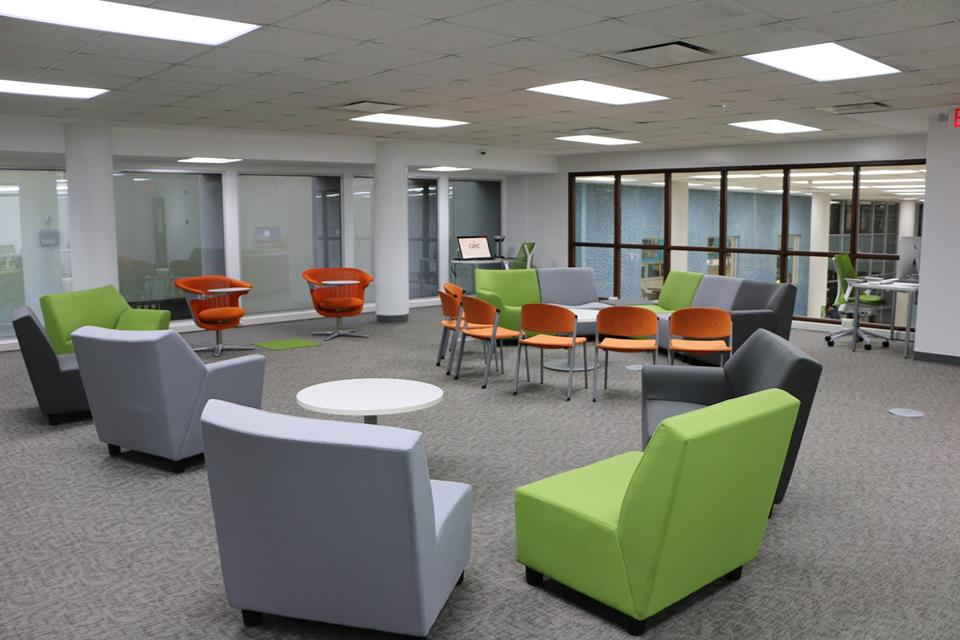
\includegraphics[width=.8\linewidth]{images/2}  
  \caption{Put your sub-caption here}
  \label{fig:sub-firstfirst}
\end{subfigure}
\begin{subfigure}{.5\textwidth}
  \centering
  % include second image
  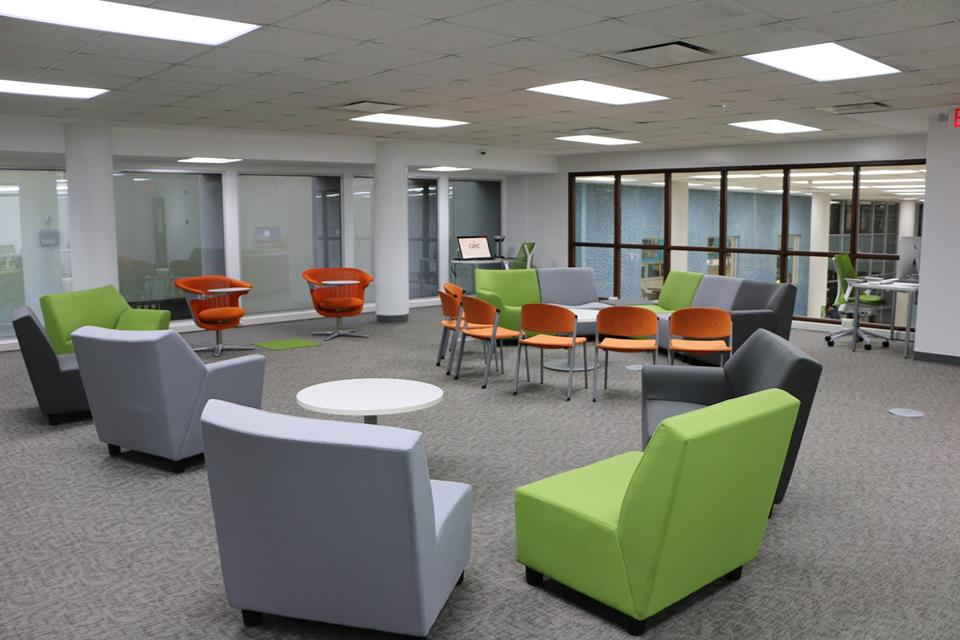
\includegraphics[width=.8\linewidth]{images/2}  
  \caption{Put your sub-caption here}
  \label{fig:sub-secondsecond}
\end{subfigure}
\begin{subfigure}{.5\textwidth}
  \centering
  % include third image
  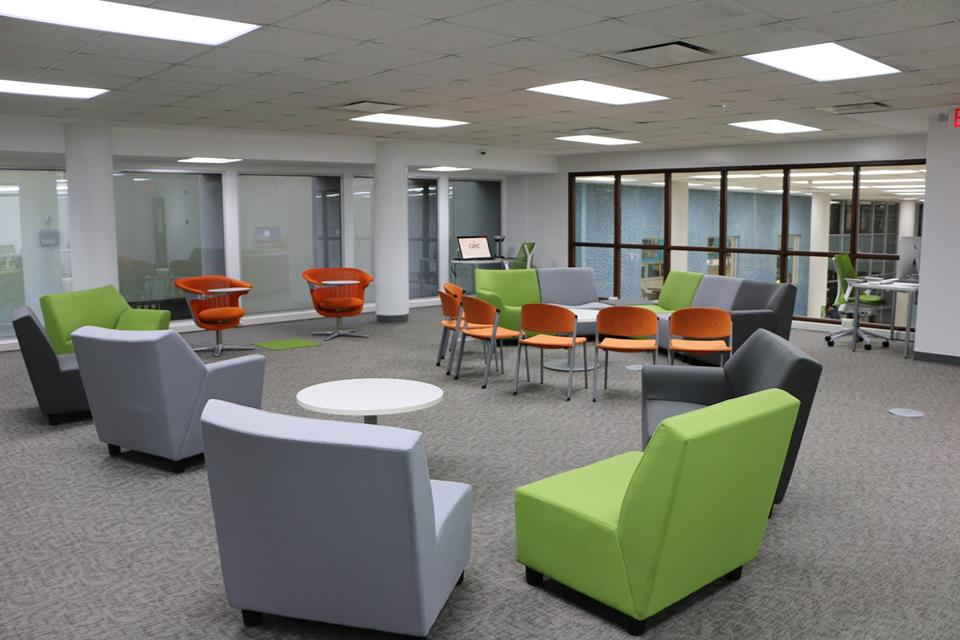
\includegraphics[width=.8\linewidth]{images/2}  
  \caption{Put your sub-caption here}
  \label{fig:sub-thirdthird}
\end{subfigure}
\begin{subfigure}{.5\textwidth}
  \centering
  % include fourth image
  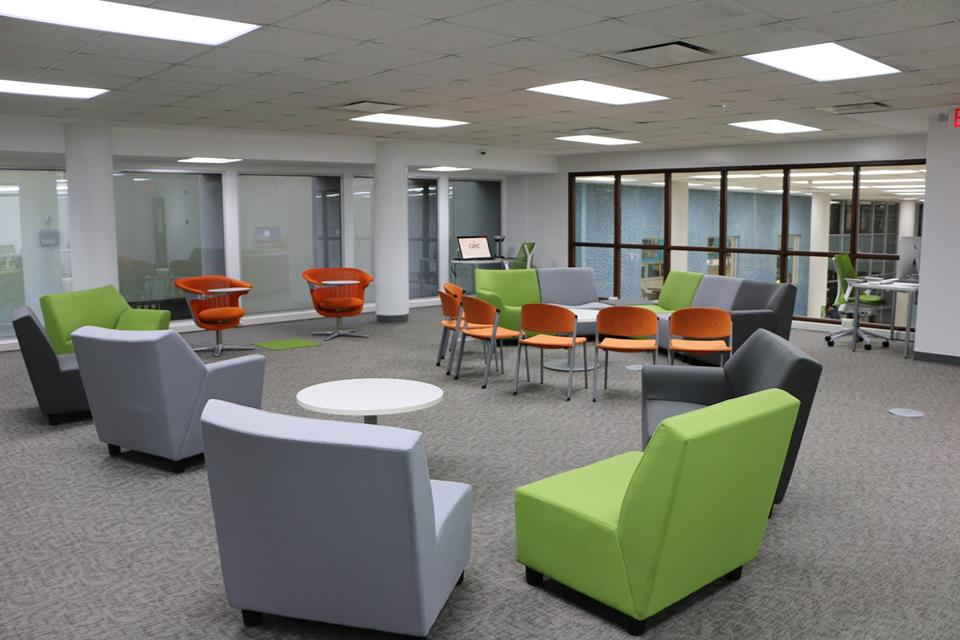
\includegraphics[width=.8\linewidth]{images/2}  
  \caption{Put your sub-caption here}
  \label{fig:sub-fourthfourth}
\end{subfigure}
\caption{Put your caption here}
\label{fig:fig}
\end{figure}

\section{Plotting Graphs}

\noindent You can import graphs as images, but you can also plot graphs in \LaTeX\ using pgfplots. This is a visualization tool to make it simpler to include plots in your documents. The basic idea is that you provide the input data/formula and pgfplots does the rest. You are welcome to experiment with this package, but really, but please, just use excel and export the image! A sample graph is shown in Figures \ref{fig:my_label} and \ref{fig:my_label2}. For additional examples, go to: \textbf{http://pgfplots.sourceforge.net/gallery.html}.

\begin{figure}[!ht]
    \centering
    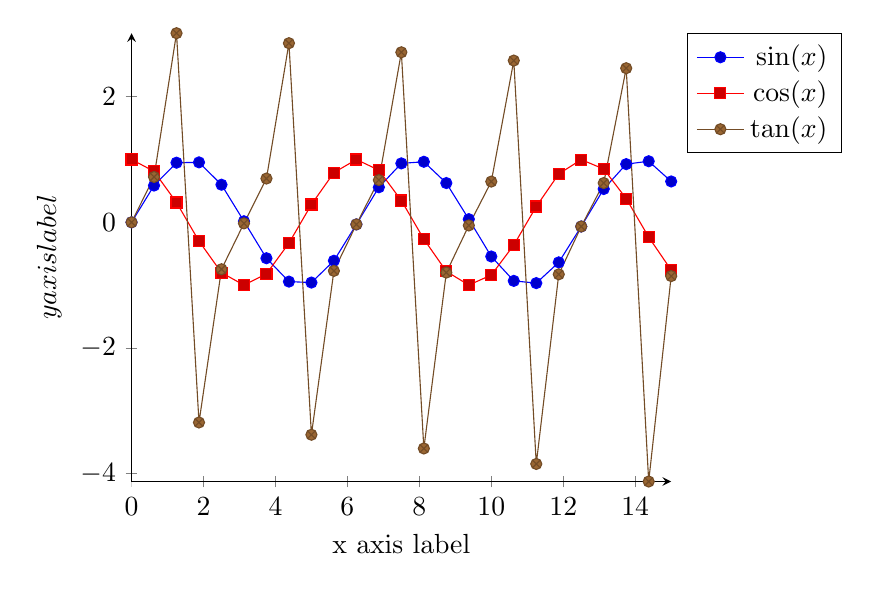
\begin{tikzpicture}
        \begin{axis}[domain=0:15,axis lines = left,
            xlabel = x axis label, %para texto
            ylabel = {\(y axis label\)}, %para notacion matematica
            legend style={cells={anchor=east},legend pos=outer north east}
	]
        \addplot {sin(deg(x))}; 
        \addplot {cos(deg(x))}; 
        \addplot {tan(deg(x))}; 
        \legend{$\sin(x)$,$\cos(x)$,$\tan(x)$}
        \end{axis}
    \end{tikzpicture}
    \caption{Put your Caption}
    \label{fig:my_label}
\end{figure}

\begin{figure}[!ht]
    \centering
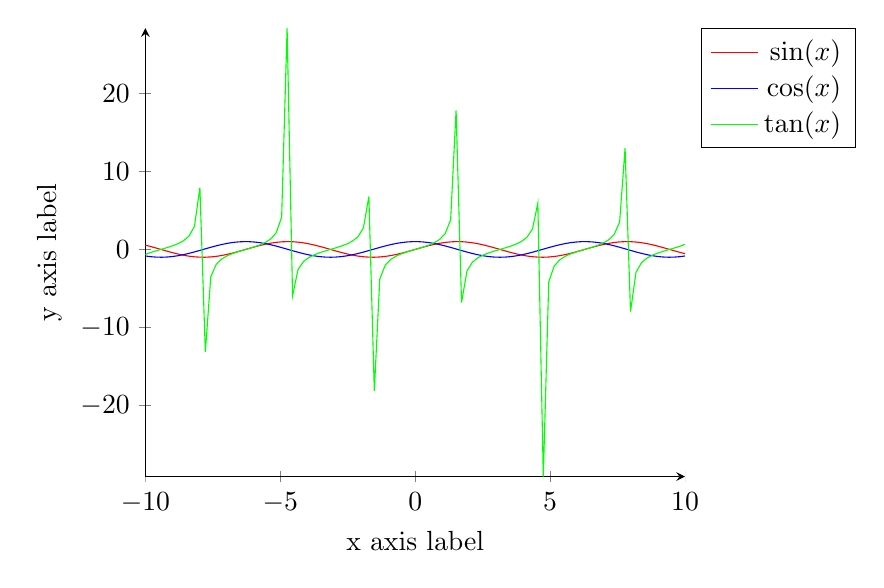
\begin{tikzpicture}
\begin{axis}[
    axis lines = left,
    xlabel = x axis label,
    ylabel = y axis label,
    legend style={
		cells={anchor=east},
		legend pos=outer north east}
]
%Plot1
\addplot [
    domain=-10:10, 
    samples=100, 
    color=red,
]
{sin(deg(x))};

%Plot2
\addplot [
    domain=-10:10, 
    samples=100, 
    color=blue,
    ]
{cos(deg(x))};

%plot3
\addplot [
    domain=-10:10, 
    samples=100, 
    color=green,
]
{tan(deg(x))};

%legend
\legend{$\sin(x)$,$\cos(x)$,$\tan(x)$}
legend pos=outer north east

\end{axis}
\end{tikzpicture}
\caption{Put another Caption}
    \label{fig:my_label2}
\end{figure}


%EQUATION EXAMPLES___________________________________________________________________________
\newpage
\section{Typing Equations in \LaTeX}

\noindent Writing equations is a bit complicated at first. It will become second nature once you get used to the symbols used. Equations are written between \textbf{begin equation and end equation} commands, and are referenced using theref command and the equation label, as in equation \ref{int1}:

\begin{equation}
\label{int1}
\int_{0}^{5}{\frac{2}{3}x}\ dx
\end{equation}

\noindent  You have several options for incorporating your equations in \LaTeX\ if you don't want to type them in the editor. Equation \ref{int1} was typed in MS Word Equation Editor and copied/pasted here. You can also use online equation converter tools, such as: \newline
 https://www.hostmath.com or https://latex.codecogs.com/eqneditor/editor.php.

\begin{equation}
\label{frac}
\frac{-b\pm\sqrt{b^2-4ac}}{2a}
\end{equation}


\begin{equation}
\label{int2}
\int_{0}^{\infty}x^{2}\ dx
\end{equation}



\subsection{Subsection}
\noindent \lipsum[1][1-3] %WRITE HERE

\subsection{Subsection}

\noindent \lipsum[1][4-6] %WRITE HERE

\chapter{Tables in \LaTeX}  

\section{How to Incorporate Tables}
\noindent Tables can be typed directly in the editor, but it's tedious, time-consuming, and can lead to errors. The easiest way to format a table to use in \LaTeX\ is to simply type it in MS Excel and convert to \LaTeX\ using \textbf{Excel2LATEX}: https://ctan.org/tex-archive/support/excel2latex. Download the zip file, unzip, run the .xla file and you're ready to go! Type your data on MS Excel, go to Add-ins, click on the Excel@LATEX icon. A window with some options will appear. Click on 'Copy to clipboard' and paste it in your \LaTeX\ document. You must enable macros for the add-in to work. Be sure to format the table as you want it to appear in your document. You can reference tables the same way as images, but using the \textbf{ref command and tab}, as seen in Table \ref{tab:table2}.
% Table generated by Excel2LaTeX from sheet 'Sheet1'
\begin{table}[htbp]
  \centering
  \caption{A centered random table}
    \begin{tabular}{ccc}
    Material & Weight (lb) & Height (ft) \\
    1     & 4.5   & 2 \\
    2     & 3.1   & 3 \\
    3     & 6.8   & 4.5 \\
    4     & 9.8   & 10 \\
    \end{tabular}%
  \label{tab:table1}%
\end{table}%https://www.overleaf.com/project/5faa3f6b47f4c254f5e0c64e

\noindent Including centering and borders/lines.

% Table generated by Excel2LaTeX from sheet 'Sheet1'
\begin{table}[htbp]
  \centering
  \caption{This looks weird}
    \begin{tabular}{|c|c|c|}
    \toprule
    \textbf{Material} & \textbf{Weight (lb)} & \textbf{Height (ft)} \\
    \midrule
    1     & 4.5   & 2 \\
    \midrule
    2     & 3.1   & 3 \\
    \midrule
    3     & 6.8   & 4.5 \\
    \midrule
    4     & 9.8   & 10 \\
    \bottomrule
    \end{tabular}%
  \label{tab:table3}%
\end{table}%

\noindent That looks bad, so sub the top, mid and bottomrule for hline.

% Table generated by Excel2LaTeX from sheet 'Sheet1'
\begin{table}[htbp]
  \centering
  \caption{This is better!}
    \begin{tabular}{|c|c|c|}
    \hline
    \textbf{Material} & \textbf{Weight (lb)} & \textbf{Height (ft)} \\
    \hline
    1     & 4.5   & 2 \\
    \hline
    2     & 3.1   & 3 \\
    \hline
    3     & 6.8   & 4.5 \\
    \hline
    4     & 9.8   & 10 \\
    \hline
    \end{tabular}%
  \label{tab:table2}%
\end{table}%


\noindent Or use thin lines instead.

% Table generated by Excel2LaTeX from sheet 'Sheet1'
\begin{table}[htbp]
  \centering
  \caption{This is best!}
    \begin{tabular}{ccc}
    \toprule
    \textbf{Material} & \textbf{Weight (lb)} & \textbf{Height (ft)} \\
    \midrule
    1     & 4.5   & 2 \\
    2     & 3.1   & 3 \\
    3     & 6.8   & 4.5 \\
    4     & 9.8   & 10 \\
    \bottomrule
    \end{tabular}%
  \label{tab:table4}%
\end{table}%







\subsection{Bigger Tables}
\noindent For tables that don't fit the width of the paper, use the \textbf{landscape command}, as shown below:

\begin{landscape}
\noindent Tables may be too big, so you can use footnotesize to make the font smaller, like in Table \ref{tab:table6}.
% Table generated by Excel2LaTeX from sheet 'Sheet1'
\begin{table}[htbp]
\footnotesize
  \centering
  \caption{You can use the footnotesize command to make the font smaller}
\begin{tabular}{ccccc}
\addlinespace
\toprule
    Temp (C) & Composition (mole\%) & Tf (C) & Heat of Fusion (kJ/kg) & Relative Cost \\
    \midrule
    367   & NaOH, NaCl (20) & 370   & 370   & 1.001 \\
          & KOH   & 360   & 167   & 4.39 \\
    347   & \ce{KNO3}, KBr (10), KCl (10) & 342   & 140   & 4.04 \\
          & NaCl, KCl (24), LiCl (43) & 346   & 281   & 5.44 \\
    328   & \ce{KNO3}  & 337   & 116   & 3.8 \\
          & \ce{KNO3}, KCl (6) & 320   & 150   & 3.33 \\
          & NaOH  & 318   & 158   & 2.78 \\
          &       & 286-299 & 3162  & 1.2 \\
    308   & NaCl,  NaOH (93.7) & 314   & -     & - \\
          & \ce{NaNO3} & 310   & 174   & 1.35 \\
          & NaF, \ce{NaNO3} (96.5) & 304   & -     & - \\
          & LiOH, KOH (60) & 314   & 341   & 3.57 \\
    289   & \ce{Na2SO4}, NaCl (8.4), \ce{NaNO3} (86.3) & 287   & 176   & 1.3 \\
          & \ce{NaNO3}, NaCl (6.4) & 284   & 171   & 1.2 \\
          & \ce{KNO3}, \ce{Ba(NO3)2} (87) & 290   & 124   & 2.85 \\
          & \ce{NaNO2} & 282   & 212   & 3.33 \\
          & \ce{NaNO2}, \ce{KNO3} (45.2) & 285   & 152   & 3.61 \\
          & NaOH, NaCl (7.8), \ce{Na2CO3} (6.4) & 282   & 316   & 2.9 \\
    \bottomrule
\end{tabular}
  \label{tab:table6}
\end{table}
\normalsize
\end{landscape}



\chapter{Literature Review}  
\noindent For tips and guidelines on how to write your Literature Review, visit the GWF clinic section at: https://libguides.uprm.edu/writingclinics, Clinics 2020.

\section{Section}
\noindent \lipsum[1][1-3] %WRITE HERE

\subsection{Subsection}
\noindent \lipsum[1][3-5] %WRITE HERE

\subsubsection{Subsubsection}
\noindent \blindtext %WRITE HERE

\subsection{Subsection}
\noindent \lipsum[1][2-5] %WRITE HERE

\subsubsection{Subsubsection}
\noindent \lipsum[1][1-5] %WRITE HERE

\section{Section}
\noindent \lipsum[1][5-8] %WRITE HERE

\subsection{Subsection}
\noindent \lipsum[1][9-15] %WRITE HERE




\chapter{Methodology}  

\section{Section}
\noindent \lipsum[1][1-3] %WRITE HERE

\subsection{Subsection}
\noindent \lipsum[1][3-5] %WRITE HERE

\subsubsection{Subsubsection}
\noindent \blindtext %WRITE HERE

\subsection{Subsection}
\noindent \lipsum[1][2-5] %WRITE HERE








\chapter{Results}  

\section{Section}
\noindent \lipsum[1][1-3] %WRITE HERE

\subsection{Subsection}
\noindent \lipsum[1][3-5] %WRITE HERE

\subsubsection{Subsubsection}
\noindent \blindtext %WRITE HERE

\subsection{Subsection}
\noindent \lipsum[1][2-5] %WRITE HERE

\subsubsection{Subsubsection}
\noindent \lipsum[1][1-5] %WRITE HERE

\section{Section}
\noindent \lipsum[1][5-8] %WRITE HERE

\subsection{Subsection}
\noindent \lipsum[1][9-15] %WRITE HERE







\chapter{Conclusions}  

\section{Section}
\noindent \lipsum[1][1-5] %WRITE HERE


\noindent \lipsum[1][1-5] %WRITE HERE


\subsection{Subsection}
\noindent \lipsum[1][1-5] %WRITE HERE


\noindent \lipsum[1][1-5] %WRITE HERE

\subsection{Subsection}
\noindent \lipsum[1][1-5] %WRITE HERE


\noindent \lipsum[1][1-5] %WRITE HERE





\bibliography{references} 
\addcontentsline{toc}{chapter}{References}
\newpage


%______________APPENDICES CONTENT______________________________
% _____________APPENDIX A______________________________________
\addcontentsline{exp}{chapter}{Appendix A: MATLAB Code} %Change title of Appendix A for List of Appendices
%\example{MATLAB CODE}
%\label{1st_ex}
\chapter*{Appendix A: MATLAB Code} %Change title of Appendix A

\noindent \lipsum[1][1-20] %WRITE HERE
\noindent \lipsum[1][1-20] %WRITE HERE
\noindent \lipsum[1][1-20] %WRITE HERE


\newpage

% _____________APPENDIX B______________________________________
\addcontentsline{exp}{chapter}{Appendix B: Data} %Change title of Appendix B for List of Appendices
\chapter*{Appendix B: Data} %Change title of Appendix B
%\example{DATA}
%\label{2nd_ex}
\noindent \lipsum[1][1-3] %WRITE HERE

\newpage

% _____________APPENDIX C______________________________________
\addcontentsline{exp}{chapter}{Appendix C: More Data} %Change title of Appendix C for List of Appendices
\chapter*{Appendix C: More Data} %Change title of Appendix C
%\example{DATA}
%\label{2nd_ex}
\noindent \lipsum[1][1-3] %WRITE HERE


% _____________APPENDIX D______________________________________
\addcontentsline{exp}{chapter}{Appendix D: More Data} %Change title of Appendix D for List of Appendices
\chapter*{Appendix D: More Data} %Change title of Appendix C
%\example{DATA}
%\label{2nd_ex}
\noindent \lipsum[1][1-3] %WRITE HERE

\end{document}